\section{Calculating the attributes}\label{sec:calculations}

Before we can properly print results in the program, we need to calculate the attributes of the different routes.
This is a relatively difficult task, as we need to calculate the distance, price, \unit{CO_{2}} and comfort.
Some attributes are easier to calculate than others, but they all require some form of calculation.

Rejseplanen has systems in place to calculate some of those attributes, but the API does not provide them.
This means that we have to calculate them ourselves.
Our calculations will not be 100\% accurate, but they will be close enough for our purposes.

\subsection{Calculating distance}\label{subsec:calculating-distance}

We need the distance of a route for our calculations.
As we don't use a map API, we can't properly calculate the distance between two points.
This means that we have to ignore roads and instead calculate the distance by the train tracks.
The problem is that Rejseplanen only provides the coordinates of the stations, not the tracks.
So what we decided to do instead is to calculate the distance between the stations.
This won't account for curves along the track, as the distance is calculated as a straight line between the stations.
However, doing this for every station along the route is better than doing this for only the start and end station.
You can see an example of how the distance is going to look in Figure~\ref{fig:image-google-maps-distance-calculation}.

\begin{figure}[H]
    \centering
    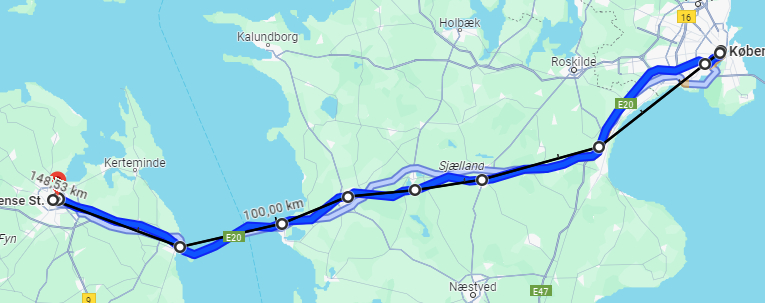
\includegraphics[width=0.8\textwidth]{images/google-maps-distance-calculation.jpg}
    \caption{A route between Copenhagen and Odense. \\ Blue line is Google Maps' distance, black line is our distance.}
    % TODO fix the text not being centered
    \label{fig:image-google-maps-distance-calculation}
\end{figure}

The way we're going to calculate the distance is by using the Haversine formula~\cite{haversine}.
The formula is used to calculate the distance between two points on a sphere, and it's used in navigation.
We'll be using the coordinates from Rejseplanen to calculate the distance between two stations.
The formula is as follows:

\begin{equation}
    haversine(\theta) = sin^{2}(\frac{\theta}{2})
\end{equation}

We can use it to calculate the distance between two points using the following formula:

\begin{equation}
    (\frac{d}{r}) = haversine(\phi_{2} - \phi_{1}) + cos(\phi_{1}) \times cos(\phi_{2}) \times haversine(\lambda_{2} - \lambda_{1})
\end{equation}

Where $\phi$ is the latitude, $\lambda$ is the longitude, $d$ is the distance and $r$ is the radius of the Earth,
which is 6371 km.

\subsection{Calculating price}\label{subsec:calculating-price}

Calculating the price is a lot more difficult than calculating the distance.
As Denmark is divided into zones, the price is calculated based on how many zones you travel through.
The price is also affected based on a number of different variables, such as age, region, occupation and more.
For our program, we decided to calculate the prices for Pendlerkort and Ungdomskort.

\subsubsection{Zones}

First thing we need to do is to figure out how many zones a route goes through.
Unfortunately, Rejseplanen's API does not provide any information about how many zones a route goes through.
What we decided to do instead is to find the average size for a zone.
As the zones are not all the same size, the number of zones a route passes through may be slightly off.
But this is the best we can do with the current circumstances.

First we started by picking two stations and counted how many zones the route goes through using DSB's zone
map~\cite{price_zones}.
We then used Google Maps to calculate the distance along the tracks between two stations, and we noted it down.
Finally, we divided the distance by the number of zones to get the average size of a zone along the route.

\begin{figure}[H]
    \centering
    \noindent
    \begin{tabular}{ || c | c | c || }
        \hline
        Route & Zones and distance & Zone size \\
        \hline\hline
        Korsør to Ringsted & 5 zones 45 km & 9 km per zone \\
        \hline
        Ringsted to Køge Nord & 6 zones 30 km & 5 km per zone \\
        \hline
        Kalundborg to Holbæk & 7 zones 45 km & 6.4 km per zone \\
        \hline
        Frederikssund to Kbh & 10 zones 23 km & 2.3 km per zone \\
        \hline
        Voldingborg to Ringsted & 8 zones 52 km & 6.5 km per zone \\
        \hline\hline
        Zone Averages & & 6 km per zone \\
        \hline
    \end{tabular}
    \caption{Table of our calculations of zone size averages.}
    \label{fig:table-zone-size-averages}
\end{figure}

From Figure~\ref{fig:table-zone-size-averages} we determined that the average size of a zone is roughly about 6
kilometers.
But as you can see, the sizes of zones varies a lot.
This is unfortunate for us, as it means that the number of zones a route goes through may be inaccurate.

\subsubsection{Pendlerkort price}

The way we're going to calculate the price will is by figuring out the price for Pendlerkort.
This card allows commuters to freely travel between set amount of zones, be that with bus or train.
Rejseplanen has a website where the user can input their route, and it'll calculate the price for the
Pendlerkort~\cite{price_calculator}.
We then took the results and compared them to the price chart provided by DSB~\cite{price_sheet}.
Our calculations can be found in Figure~\ref{fig:table-rejseplanen-price-calculations} and
Figure~\ref{fig:image-dsb-pendlerkort-pris}.
The results are accurate enough that we deemed them good enough for our purposes.

\begin{figure}[H]
    \centering
    \noindent
    \begin{tabular}{ || c | c || }
        \hline
        Route & Zones and price \\
        \hline\hline
        Odense to København & 30 zones 3750 kr \\
        \hline
        Køge Nord to København & 9 zones 1470 kr \\
        \hline
        Græsted to Vordingborg & 18 zones 3000 kr \\
        \hline
        Aarhus to København & 51 zones 4590 kr \\
        \hline
    \end{tabular}
    \caption{Table of Rejseplanen's price calculations.}
    \label{fig:table-rejseplanen-price-calculations}
\end{figure}

\begin{figure}[H]
    \centering
    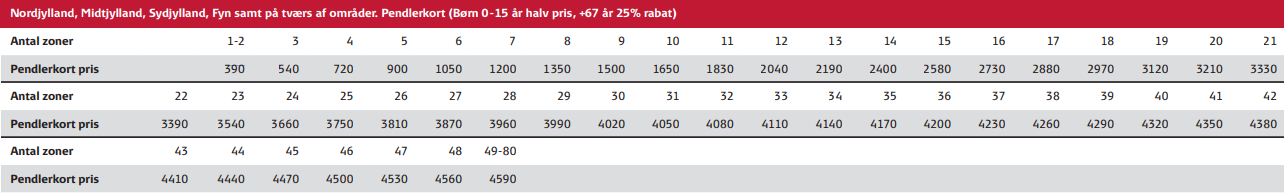
\includegraphics[width=1\textwidth]{images/dsb-pendlerkort-pris.jpg}
    \caption{Price of Pendlerkort per zones.}
    \label{fig:image-dsb-pendlerkort-pris}
\end{figure}

From what it seems, the price table is not recursive, so we can't implement a function to calculate the price.
Instead, we can save the table in the program and reference it when we need to find the price.
This allows us to have a pretty accurate price chart as long as the number of zones is accurate.

\subsubsection{Ungdomskort price}

Ungdomskort is a type op Pendlerkort that is primarily aimed at young people or students.
The price is significantly lower than Pendlerkort, so we deemed it necessary to implement it in our program.
The program would ask the user if they're a student, and if they are, the next calculation will be executed.
Calculating the price for Ungdomskort is a lot easier than Pendlerkort, as the method is listed on their
website~\cite{price_ung}.

The price is calculated by taking the equivalent price for a Pendlerkort and then taking 2487 kr from it.
Then the result is halved, and finally 663 kr is added to the result.
Here's an example for a Pendlerkort between Odense and Copenhagen, that costs 3750 kr:

\begin{equation}
    \frac{3750 - 2487}{2} + 663 = 1294 \text{kr}
\end{equation}

As a member in our group travels that same distance with an Ungdomskort, we can confirm this result to be accurate.

\subsubsection{Car and bike price}

As we're calculating the price for public transportation, we also need to calculate the price for cars and bikes.
Of course, we'll be looking into the prices assuming that the user owns a car or a bike.
What we're looking into is the price of gas or electricity, insurance and maintenance.
Do note that pricing can vary a lot depending on different circumstances, so we'll be looking into the average prices.

First we'll look into the prices for gas.
According to Global Petrol Prices, the average price for gas in Denmark is 12.20 kr per liter~\cite{price_gas}, however
looking at the graph, it seems that recently the prices have been around 14 kr, so we'll choose that number for our
calculations.
Since we ask the user to input their car's fuel efficiency, we can use that in our calculations, otherwise we can use
the average fuel efficiency, which is 24 MPG (Miles Per Gallon)~\cite{price_mpg} and equals to 10.2 km per liter.
This will be the default in case the user does not input their car's fuel efficiency.
Our program will take the distance and divide it by the fuel efficiency, and then multiply it by the price of gas.
This will give us the price for gas for the route.
We'll then have to multiply the price by two, as the user will have to travel back home.
And finally, we'll have to multiply the price by 20, as the user will have to travel for the duration of work month.
Here's an example of a commute that's 30 km long with a fuel efficiency of 17 km per liter and a gas price of 14 kr

\begin{equation}
    \frac{30}{17} \times 14 \times 40 = 988 \text{kr}
\end{equation}

We can again confirm this result to be accurate.

While electric cars don't require gas, they do require electricity.
The most popular electric car in Denmark, the Tesla Model 3, happens to be the most economical electric car with an
efficiency of 142 MPG-e (Miles Per Gallon equivalent), which is about 60 km per liter equivalent~\cite{price_el}.
Of course, electric cars don't use liters or gallons, so we say ``equivalent'' in this case.
One gallon is the equivalent of 33.7 kWh~\cite{price_mpge}, which is 8.9 kWh per liter.
With that in mind, we can use the price of electricity in Denmark, which is 2.8 kr per kWh~\cite{price_energy}, to
figure out that the cost per km for electric cars is 24.9 kr.
And we can use the same calculations as we did for gas to figure out the price for electricity.

Next we'll look into the price of insurance and maintenance.
A big factor for the insurance price depends on the type of subscription the user has, but the average cost is roughly
250 kr per month~\cite{price_insurance}.
When it comes to maintenance, the average cost is about \$1064~\cite{price_repair}, which equals to 600 kr per month.
This amounts for 850 kr that the user has to pay on top of the gas or electricity prices for the month.

Bikes in comparison are a lot cheaper, as they don't require insurance or gas.
However, they do require maintenance.
But compared to cars, maintenance for bikes is also a lot cheaper.
According to The Pro's Closet, they've estimated that the average cost of maintenance for a road bike is about \$185 per
year~\cite{price_bike}.
This converts to about 1200 kr per year, which is 100 kr per month.
This is a lot cheaper than cars, but it's still a cost that needs to be accounted for.

\subsection{Calculating time}\label{subsec:calculating-time}

Calculating the time is marginably easier than calculating the distance, but only for trains.
Rejseplanen provides a time for when the train arrives at the station, and when it departs.
So for a train route, we can simply find the difference in time and that'll be our time for the route.
However, for cars and bikes, we need to calculate the time ourselves.
We can do this by taking the distance and dividing it by the average speed of a car or bike.
As we're looking into long distances, we're expecting that the user will be using the highway.
But the user will also have to spend some time in the city, so we'll have to take that into account as well.

We expect that the user will spend around 15 minutes to get out of the city, and 15 minutes to get into the next city.
So for the first 30 minutes, we'll be using the average speed of a car in the city, and afterwards we'll be using the
average speed of a car on the highway.
The average speed of a car on the highway is about 120 km/h~\cite{time_highway}, and the average speed of a car in
the city is about 35 km/h~\cite{time_city}.
This would mean that for the first 17.5 km we'd divide by 35 and for the remaining we'll divide by 120.
Which will result in the number of hours the car ride will take.
We can also find the number of minutes by multiplying the decimal by 60.

Depending on the distance, bike and walking time might be unrealistic.
This is already the case with for example Google Maps, where the time it takes to walk a distance does not include
breaks or sleep, resulting in a vastly smaller time estimate.
A 100 km trip is estimated to take 23 hours, but it'll realisically take more than 2 days at least.
This could be misleading at longer distances, because 24 hours converts to 1 day.
We would keep this behaviour, however we won't round the time up to days.
Walk and bike speed can vary by age and sex, but we decided to settle on an average of 4.6 km/h, which should be
accurate for people up to 50 years of age~\cite{time_walk}.
As for biking, the speed can vary by the bike and the biker's experience too.
We settled for 17.5 km/h, which is the average speed for a normal bike tour~\cite{time_bike}.
The calculation process is similar to that for cars.

\subsection{Calculating \unit{CO_{2}} emission}\label{subsec:calculating-co2-emission}

The final attribute we need to calculate is the \unit{CO_{2}} emission.
Luckily, public companies have to report their \unit{CO_{2}} emissions, so we can use that in our calculations.
The list below is a sample of the different types of public transport vehicles and their \unit{CO_{2}} emissions pr.
person pr. kilometer (km) as seen in~\ref{tab:emissions}.

\begin{table}[H]
    \centering
    \begin{tabular}{ || c | c || }
        \hline
        Vehicle type & \unit{CO_{2}} pr. person pr. km \\
        \hline\hline
        S-train & 14 gram~\cite{dsb2023} \\
        \hline
        Regional train & 38 gram~\cite{dsb2023} \\
        \hline
        InterCity train & 29 gram~\cite{dsb2023} \\
        \hline
        Speed train & 37 gram~\cite{dsb2023} \\
        \hline
        Long distance bus & 23 gram~\cite{cowi2022} \\
        \hline
        City bus & 10 gram~\cite{ntm2023} \\
        \hline
    \end{tabular}
    \caption{\unit{CO_{2}} pr. person pr. km. pr. vehicle type.}
    \label{tab:emissions}
\end{table}

Since the data is per km, we can multiply the distance by the \unit{CO_{2}} emission to get the total \unit{CO_{2}}.
And multiply by 40, similar to how we did in the price calculation, to get the \unit{CO_{2}} emission for a month.
The number will be quite large, as it is in grams, so we'll have to divide by 1000 to get the number in kilograms.
And with that, we're finished with all the calculations.

% \subsection{Calculating comfort value}\label{subsec:calculating-comfort-value}
% TODO Optional: Add comfort as an attribute
